\section{CW-complexes}

There are various ways to model geometrically interesting spaces. 
Manifolds provide one important model, well suited to analysis.  
Another model, one we have not talked 
about, is given by simplicial complexes. It's very combinatorial,
and constructing a simplicial complex model for a given space involves
making a lot of choices that are combinatorial rather than topological
in character. A more flexible model, one more closely reflecting topological
information, is given by the theory of CW-complexes. 

In building up a space as a CW-complex, we will successively ``glue'' cells
onto what has been already built. This is a general construction. 

Suppose we have a pair $(B,A)$, and a map $f:A\to X$. Define a space
$X\cup_f B$ (or $X\cup_A B$) in the diagram
\begin{equation*}
\xymatrix{A\ar[r]^f\ar@{^(->}[d] & X\ar[d]\\
B\ar[r] & X\cup_f B}
\end{equation*}
by
\[
X\cup_f B=X\sqcup B/\sim
\]
where the equivalence relation is generated by requiring that $a\sim f(a)$ 
for all $a\in A$. We say that we have ``attached $B$ to $X$ along $f$ (or 
along $A$).'' 

There are two kinds of equivalence classes in $X\cup_fB$: (1) singletons containing elements of $B-A$, and (2) $\{x\}\sqcup f^{-1}(x)$ for $x\in X$.
The topology on $X\cup_fB$ is the quotient topology, and is characterized
by a universal property: any solid-arrow commutative diagram
\begin{equation*}
\xymatrix{A\ar[r]^f\ar@{^(->}[d] & X\ar[d]^j\ar[ddr]^{\overline{j}} & \\
B\ar[r]\ar[drr]_{\overline{g}} & X\cup_f B\ar@{-->}[dr] & \\
 & & Y}
\end{equation*}
can be uniquely filled in. It's a ``push-out.''
\begin{example}
If $X=\ast$, then $\ast\cup_f B=B/A$.
\end{example}
\begin{example}
If $A=\varnothing$, then $X\cup_fB$ is the coproduct $X\sqcup B$. 
\end{example}
\begin{example}
If both, 
\[
B/\varnothing=\ast\cup_\varnothing B=\ast\sqcup B\,.
\]
For example, $\varnothing/\varnothing=\ast$. 
This is creation from nothing. We won't get into the religious ramifications.
\end{example}
\begin{example}[Attaching a cell]
A basic collection of pairs of spaces is given by the disks relative to their
boundaries: $(D^n,S^{n-1})$. (Recall that $S^{-1}=\varnothing$.) In this
context, $D^n$ is called an ``$n$-cell,'' and a map $f:S^{n-1}\to X$ allows
us to attach an $n$-cell to $X$, to form 
\begin{equation*}
\xymatrix{S^{n-1}\ar[r]^f\ar@{^(->}[d] & X\ar[d]\\
D^n\ar[r] & X\cup_f D^n}
\end{equation*}
You might want to generalize this a little bit, and attach a bunch of $n$-cells all at once:
\begin{equation*}
\xymatrix{\coprod_{\alpha\in A}S^{n-1}_\alpha\ar[r]^f\ar@{^(->}[d] & X\ar[d]\\
\coprod_{\alpha\in A}D^n_\alpha\ar[r] & X\cup_f \coprod_{\alpha\in A}D^n_\alpha}
\end{equation*}
\end{example}
What are some examples? When $n=0$, $(D^0,S^{-1})=(\ast,\varnothing)$, so 
you are just adding a discrete set to $X$:
\[
X\cup_f\coprod_{\alpha\in A}D^0=X\sqcup A
\]
More interesting: Let's attach two 1-cells to a point:
\begin{equation*}
\xymatrix{S^0\sqcup S^0\ar[r]^f\ar@{^(->}[d] & \ast\ar[d]\\
D^1\sqcup D^1\ar[r] & \ast\cup_f (D^1\sqcup D^1)}
\end{equation*}
Again there's just one choice for $f$, and 
$\ast\cup_f(D^1\sqcup D^1)$ is a figure $8$, because you start with 
two $1$-disks and identify the four boundary points together. Let me write 
$S^1\vee S^1$ for this space. We can go on and attach a single 2-cell to 
manufacture a torus. Think of the figure 8 as the perimeter of a square with opposite sides identified.

\medskip
\begin{center}
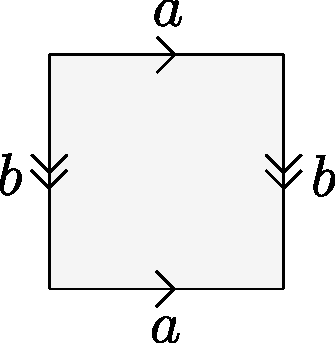
\includegraphics[width=1.75in]{905/Figures/14-torus-CW-structure.pdf}
\end{center}

The inside of the square is a 2-cell, attached to the perimeter by a map I'll denote by $aba^{-1}b^{-1}$: 
\begin{equation*}
\xymatrix{S^1\ar[r]^{aba^{-1}b^{-1}}\ar@{^(->}[d] & S^1\vee S^1\ar[d]\\
D^2\ar[r] & (S^1\vee S^1)\cup_f D^2=T^2\,.
}\end{equation*}

This example illuminates the following definition.

\begin{definition}
A \emph{CW-complex} is a space $X$ equipped with a sequence of subspaces 
\[
\varnothing=\Sk_{-1}X\subseteq\Sk_0X\subseteq\Sk_1X\subseteq\cdots\subseteq X
\]
such that 
\begin{itemize}
\item $X$ is the union of the $\Sk_nX$'s, and 
\item for all $n$, there is a pushout diagram like this:
\begin{equation*}
\xymatrix{\coprod_{\alpha\in A_n}S^{n-1}_\alpha\ar[r]^-{f_n}\ar@{^(->}[d] 
& \Sk_{n-1}X\ar[d]\\
\coprod_{\alpha\in A_n}D^n_\alpha\ar[r]^-{g_n} & \Sk_nX}\,.
\end{equation*}
\end{itemize}
\end{definition}
The subspace $\Sk_nX$ is the $n$-{\em skeleton} of $X$. 
Sometimes it's convenent to use the alternate notation $X_n$ 
for the $n$-skeleton.
The first condition is intended topologically, so that a subset of $X$ is open if and only if its intersection with each $\Sk_nX$ is open; or, equivalently, a map $f:X\to Y$ is continuous if and only if its restriction to each $\Sk_nX$ is continuous. The maps $f_n$ are the {\em attaching maps} and the maps $g_n$ are {\em characteristic maps}. 

\begin{example}
We just constructed the torus as a CW complex with $\Sk_0T^2=\ast$, $\Sk_1T^2=S^1\vee S^1$, and $\Sk_2T^2=T^2$.
\end{example}
\begin{definition}
A CW-complex is \emph{finite-dimensional} if $\Sk_nX=X$ for some $n$;
of \emph{finite type} if each $A_n$ is finite, i.e., finitely many cell in each dimension; and \emph{finite} if it's finite-dimensional and of finite type.
\end{definition}
The {\em dimension} of a CW complex is the largest $n$ for which there are 
$n$-cells. This is not obviously a topological invariant, but, have no fear,
it turns out that it is.

In ``CW,'' the ``C'' is for cell, and the ``W'' is for weak, because of the topology on a CW-complex. This definition is due to J. H. C. Whitehead. Here are a couple of important facts about them. 
\begin{theorem}
Any CW-complex is Hausdorff, and it's compact if and only if it's finite. \\
Any compact smooth manifold admits a CW structure.
\end{theorem}
\begin{proof} See \cite{bredon} Prop. IV.8.1, \cite{hatcher} Prop. A.3.
\end{proof}

